\section{Results and Analysis}

This study assessed eight tokenizers on a Turkish MMLU dataset of 1,605,376 characters and 198,193 words \cite{bayram_turkish_nodate}. To capture both linguistic fidelity and computational effectiveness, we measured Turkish Token Percentage (TR \%) and Pure Token Percentage (Pure \%), along with processing time, parameter size, and MMLU scores. Incorporating model size into the analysis provides a nuanced view of the trade-offs involved in designing tokenizers for morphologically rich languages.

\begin{table}[h]
\centering
\caption{Tokenizer Benchmark Results}
\label{tab:tokenizer-benchmark}
\resizebox{\textwidth}{!}{
\begin{tabular}{|l|c|c|c|c|c|c|c|c|}
\hline
\textbf{Metric} & \textbf{gemma-2} & \textbf{llama-3.1} & \textbf{EuroLLM} & \textbf{Qwen2.5} & \textbf{aya-exp} & \textbf{Mistral} & \textbf{Phi3.5} & \textbf{gpt4o} \\ \hline
Model Params (B) & 27.2 & 70.6 & 9.2 & 7.6 & 32.3 & 12.2 & 3.8 & Unknown \\ \hline
MMLU Score (\%) & 72.10 & 70.42 & 51.29 & 61.68 & 70.66 & 46.89 & 29.37 & 84.84 \\ \hline
Vocab Size & 256,000 & 128,256 & 128,000 & 151,665 & 255,029 & 131,072 & 32,011 & 200,019 \\ \hline
Token Count & 497,015 & 488,535 & 497,173 & 561,866 & 434,526 & 534,930 & 803,971 & 491,137 \\ \hline
Time (s) & 2.95 & 3.12 & 3.20 & 3.31 & 2.77 & 3.14 & 4.55 & 0.51 \\ \hline
Unique Tokens & 6,383 & 6,823 & 5,226 & 5,752 & 8,562 & 4,354 & 3,640 & 7,615 \\ \hline
Turkish Tokens & 3,104 & 3,125 & 2,457 & 2,320 & 4,338 & 1,971 & 1,599 & 3,209 \\ \hline
TR \% & 48.63 & 45.80 & 47.01 & 40.33 & 50.67 & 45.27 & 43.93 & 42.14 \\ \hline
Pure Tokens & 2,365 & 2,109 & 1,838 & 1,734 & 2,822 & 1,571 & 1,253 & 2,184 \\ \hline
Pure \% & 37.05 & 30.91 & 35.17 & 30.15 & 32.96 & 36.08 & 34.42 & 28.68 \\ \hline
\end{tabular}
}
\end{table}

Table~\ref{tab:tokenizer-benchmark} summarizes these metrics, illustrating how vocabulary size, token counts, runtime, and language-specific alignment interact with downstream performance. Notably, larger parameter sizes do not guarantee superior results. For instance, \texttt{gemma-2} (27.2B parameters) outperformed the considerably larger \texttt{llama-3.1} (70.6B parameters) in Turkish MMLU accuracy, indicating that \texttt{gemma-2}’s tokenizer is better tuned to Turkish morphology. This contrasts with their English MMLU standings, where \texttt{llama-3.1} excels \cite{ai_llama_nodate}, underscoring the language-dependence of tokenizer effectiveness.

\texttt{gemma-2} achieved higher TR \% (48.63\%) and Pure \% (37.05\%) than \texttt{llama-3.1} (45.80\% TR, 30.91\% Pure), emphasizing the importance of language-specific tokenization in capturing morphological structure. Although \texttt{aya-expanse} (32.3B) recorded the highest TR \% (50.67\%), its MMLU score (70.66\%) leaves room for improvement, demonstrating that while linguistic alignment is crucial, it must be balanced with computational efficiency and task optimization.

At the other end of the spectrum, \texttt{o200k-gpt40} achieved the highest MMLU score (84.84\%) and fastest processing time (0.51s), but with a relatively modest TR \% (42.14\%). This trade-off reflects the impact of optimization techniques like distillation and pruning \cite{lacy_gpt-4o_2024,shakrapani_gpt_nodate}, which boost performance and speed at the expense of linguistic fidelity. Similarly, smaller models such as \texttt{Mistral} (12.2B) and \texttt{Phi3.5} (3.8B) struggled on both fronts, demonstrating that limited parameter counts often require more sophisticated tokenization strategies to handle complex morphologies effectively.


Figure~\ref{fig:model_comparison} provides a multidimensional visualization of these trade-offs, plotting MMLU scores against TR \%, with marker size representing parameter count and color encoding Pure \%. This allows for a holistic comparison: models that achieve high TR \% and Pure \% tend to better capture the language’s morphological richness, while those with large parameter counts or specific optimizations may excel in overall performance yet fail to preserve linguistic integrity.

\begin{figure}[h!]
    \centering
    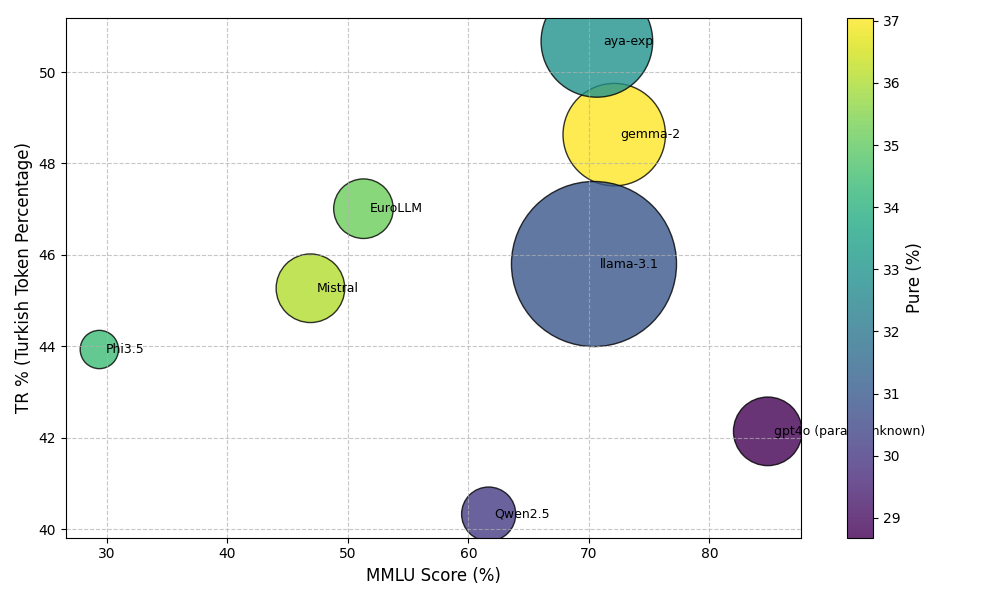
\includegraphics[width=1\textwidth]{model_comparison.png}
    \caption{
    Model Comparison: MMLU vs TR\%, Parameter Size (Unknown for gpt4o), and Pure\%
    }
    \label{fig:model_comparison}
\end{figure}

In summary, these results confirm that linguistic alignment significantly shapes downstream success in morphologically complex settings. Tailored tokenization can help smaller models compete effectively, while even large or optimized models may fall short if their tokenizers are not linguistically attuned.

\section{Yöntem}

Bu çalışma, morfolojik olarak zengin ve eklemeli dillere yönelik tokenizasyon stratejilerini değerlendirmeyi hedeflemekte olup, Türkçe bu bağlamda temsilci bir örnek olarak kullanılmaktadır. Ana odak Türkçe olsa da, yöntem diğer dillerdeki benzer tokenizasyon zorluklarına uyarlanabilir bir esneklikle tasarlanmıştır.

Bu değerlendirmeyi gerçekleştirmek için, çeşitli konuları kapsayan 6.200 çoktan seçmeli sorudan oluşan Türkçe MMLU veri seti kullanılmıştır \cite{bayram_turkish_nodate}. Bu veri seti, Hugging Face deposunda saklanan ön işlenmiş bir kaynaktan soruların ve cevapların çıkarılmasıyla hazırlanmıştır \cite{bayram_turkish_nodate}. Ortaya çıkan metin korpusu, Türkçe'de karşılaşılan çeşitli dilbilimsel yapıları geniş bir kapsama alanıyla içeren birleşik bir veri setine dönüştürülmüştür. Türkçe verileri kullanılarak geliştirilen bu çerçeve, benzer dil araçları ve kaynaklarının uygulanmasıyla diğer dillere de uyarlanabilir.

Bu çalışma kapsamında, tokenizasyonun hem hesaplama hem de dilbilimsel yönlerini değerlendirmek için çeşitli metrikler kullanılmıştır:

\textbf{Sözlük Boyutu:}  
Bir tokenizatörün üretebileceği benzersiz tokenların (ör. kelimeler, alt kelimeler, karakterler) toplam sayısını ifade eder. Örneğin, 50.000 sözlük boyutuna sahip bir tokenizatör \texttt{"cat"} veya \texttt{"run"} gibi tokenları, ayrıca \texttt{"run"} ve \texttt{"ning"} gibi alt kelime birimlerini içerebilir. Daha büyük sözlükler daha karmaşık dilbilimsel yapıları yakalayabilir, ancak aşırı büyük sözlükler karmaşıklığı ve bellek kullanımını artırabilirken, daha küçük sözlükler nadir kelimeleri yeterince temsil edemeyebilir.

\textbf{Toplam Token Sayısı:}  
Tokenizatör uygulandıktan sonra veri setinde üretilen toplam token sayısını ifade eder. Örneğin, \texttt{"I love programming languages"} cümlesi, boşluk tabanlı bir tokenizatörle [\texttt{"I"}, \texttt{"love"}, \texttt{"programming"}, \texttt{"languages"}] olarak ayrıştırıldığında dört token oluşur. Alt kelime tabanlı bir tokenizatör, [\texttt{"I"}, \texttt{"love"}, \texttt{"program"}, \texttt{"ming"}, \texttt{"languages"}] şeklinde beş token üretebilir. Daha düşük toplam token sayıları, daha kompakt temsiller anlamına gelebilir ve bu da verimliliği artırabilir.

\textbf{İşleme Süresi:}  
Veri setinin tamamını tokenize etmek için gereken süreyi (saniye cinsinden) ifade eder ve hesaplama verimliliğini yansıtır. Örneğin, bir milyon kelimelik bir korpus 3.2 saniyede işlenirse, işleme süresi 3.2 saniye olarak kaydedilir. Daha hızlı tokenizasyon, büyük ölçekli eğitimler ve gerçek zamanlı uygulamalar için avantajlıdır.

\textbf{Token Yüzdesi (\%TR):}  
Hedef dilde geçerli kelimelere veya morfemlere karşılık gelen tokenların oranını ölçen bir dilbilimsel metriktir. Örneğin, \texttt{"Cats are playing"} cümlesi [\texttt{"Ca"}, \texttt{"ts"}, \texttt{"are"}, \texttt{"play"}, \texttt{"ing"}] olarak tokenize edilirse, \texttt{"are"}, \texttt{"play"} ve \texttt{"ing"} geçerli dilbilimsel birimler olarak kabul edilir. Bu durumda:  
\[
\%TR = \frac{\text{Geçerli Tokenlar (3)}}{\text{Toplam Tokenlar (5)}} \times 100 = 60\%.
\]
Bu metrik, tokenizasyonun dilin morfolojisine uygunluğunu sağlar ve geçersiz segmentleri en aza indirir.

\textbf{Saf Token Yüzdesi (\%Pure):}  
Tokenların doğrudan anlamlı olup olmadığını ve daha küçük anlamlı parçalara ayrılıp ayrılamayacağını değerlendiren bir metriktir. Örneğin, \texttt{"The students are learning"} cümlesinde, \texttt{"The"} ve \texttt{"are"} saf tokenlardır, ancak \texttt{"students"} (\texttt{"student"} + \texttt{"s"}) ve \texttt{"learning"} (\texttt{"learn"} + \texttt{"ing"}) saf değildir, çünkü daha küçük birimlere ayrılabilirler. Eğer bir tokenizatör 100 benzersiz token üretmiş ve bunların 70’i saf token ise:  
\[
\%Pure = \frac{\text{Saf Tokenlar (70)}}{\text{Benzersiz Tokenlar (100)}} \times 100 = 70\%.
\]

Doğru morfolojik analiz ve token doğrulaması sağlamak için ITU Turkish NLP Web Service \cite{eryigit_itu_2014} ve Kalbur kütüphanesi \cite{aksoy_ahmetaxkalbur_2024} gibi dil araçlarından yararlanılmıştır. Diğer diller için benzer dil analiz araçları ve kurallara dayalı sistemler entegre edilebilir. İşleme süresi ve token sayıları gibi hesaplama metrikleri, Python betikleri ve Hugging Face Tokenizers kütüphanesi \cite{neubeck_so_2024} kullanılarak hesaplanmış ve bu, ölçeklenebilirliği ve uyarlanabilirliği sağlamıştır.

Tüm deneysel prosedürler, veri setleri ve yapılandırmalar çoğaltılabilirlik için belgelenmiştir. Bu çalışmada Türkçe birincil referans olarak kullanılmış olsa da, önerilen yöntem diğer dillere ve veri setlerine uygulanabilir bir yapı sunarak, farklı dilsel bağlamlarda tokenizasyon stratejilerini değerlendirmeye yönelik genel bir yaklaşım sunmaktadır.